\documentclass[a4paper]{article}

\input ../header
\usepackage[np]{numprint}

\setlength{\multicolsep}{2pt}

\begin{document}

\title{Sujet B -- Internet}

\pagestyle{empty}

\date{}
\author{}

\maketitle{}
\thispagestyle{empty}

\exo[2 points]\vspace*{-2mm}
\begin{enumerate}
  \item Existe-t-il une différence entre Internet et le Web ?\rep{4}
  \item Donner deux exemples de services proposés par Internet.\rep{4}
\end{enumerate}

\bigskip

\exo[3 points]\vspace*{-2mm}
\begin{enumerate}
  \item Qu'est-ce que Napster ?\rep{4}
  \item Qu'était le projet Arpanet ?\rep{4}
\end{enumerate}

\bigskip

\exo[6 points]\vspace*{-2mm}
\begin{enumerate}
  \item Qu'est-ce qu'un octet ? un gigaoctet ?\rep{4}
  \item On considère le graphique ci-dessous : 
   \begin{center}
     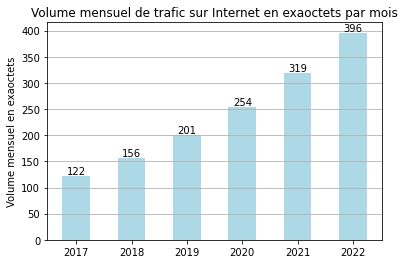
\includegraphics[width=10cm]{volume.png}
   \end{center} 
   Que signifie la valeur $254$ ?\rep{4}
  \item Retrouver le volume quotiden échangé sur Internet en 2020.\rep{10}
  \item Combien de disques durs de $2$ To sont nécessaires pour stocker ce volume de données ?\rep{4}
\end{enumerate}

\bigskip

\exo[4 points]\vspace*{-2mm}
\begin{enumerate}
  \item Comment écrit-on un commentaire en Python ?\rep{2}
  \item Le graphique de l'exercice précédent a été obtenu grâce aux lignes suivantes :
    \begin{minted}{python}
import matplotlib.pyplot as plt

annees = [2017, 2018, 2019, 2020, 2021, 2022]
volume = [122, 156, 201, 254, 319, 396]
plt.bar(annees, volume, width=0.5, color="lightblue")
plt.grid(axis="y")
plt.title("Volume mensuel de trafic sur Internet en exaoctets par mois")
plt.ylabel("Volume mensuel en exaoctets")
plt.show()
    \end{minted}
    Quelle ligne peut-on écrire afin d'ajouter une légende pour l'axe des abscisses ?\rep{3}
  \item Modifier le code précédent afin d'obtenir le graphique suivant :
    \begin{center}
      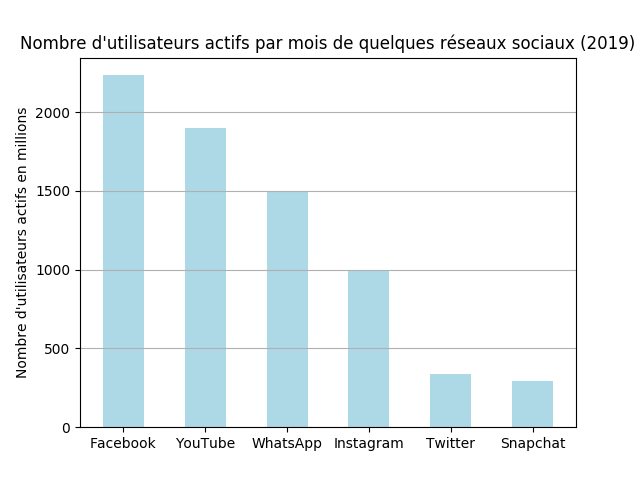
\includegraphics[width=10cm]{utilisateurs_actifs_reseaux_sociaux.png}  
    \end{center}
    \begin{center}
      \renewcommand{\arraystretch}{1.2}
      \begin{tabular}{|>{\centering}m{4cm}|*{6}{>{\centering}m{1.6cm}|}}
	\hline
	Réseau social & Facebook & YouTube & WhatsApp & Instagram & Twitter & Snapchat\tabularnewline
	\hline
	Nombre d'utilisateurs actifs par mois, en millions (2019) & $\np{2234}$ & $\np{1900}$ & $\np{1500}$ & $\np{1000}$ & $\np{335}$ & $\np{291}$\tabularnewline
	\hline
      \end{tabular}
    \end{center}
    \dotfill\rep{10}
\end{enumerate}

\end{document}
